\section{Estabilidad tractogramas}

Las Figuras \ref{fig:m1}, \ref{fig:m2} y \ref{fig:m3} muestran, para tres semillas
distintas, cinco cortes axiales del tractograma que se consigue al utilizar quince
mil part\'iculas.\\

Las Figuras \ref{fig:s1}, \ref{fig:s2} y \ref{fig:s3} muestran la varianza de 
cada voxel dentro de un mismo corte axial. La varianza se calcul\'o generando
mil tractogramas desde distinto n\'umero de streamlines. \\

La Figura \ref{fig:mv} muestra la media y varianza de los voxels $A$, $B$ y $C$
marcados en las Figuras \ref{fig:s1}, \ref{fig:s2} y \ref{fig:s3}. Estos voxels
fueron los que mayor varianza presentaron al generar tractogramas con dos mil
\textit{streamlines}.


\begin{figure}[h!]
   \centering
    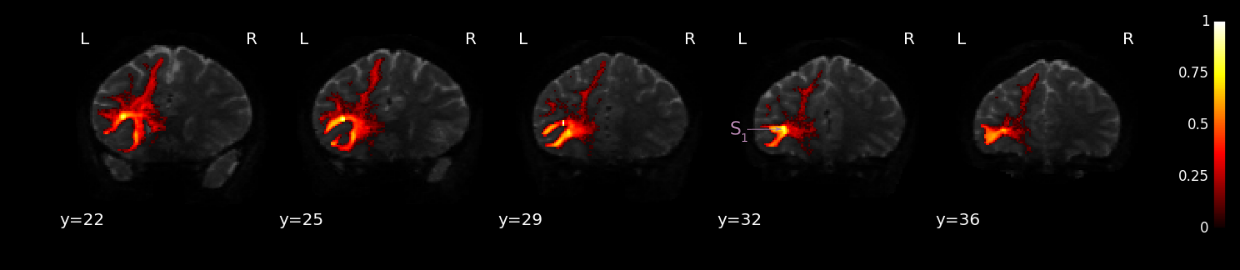
\includegraphics[width=\textwidth]{img/m1.png}
    \caption{Tractograma para la semilla $S1$ utilizando toda la muestra.}
    \label{fig:m1}
\end{figure}

\begin{figure}[h!]
   \centering
    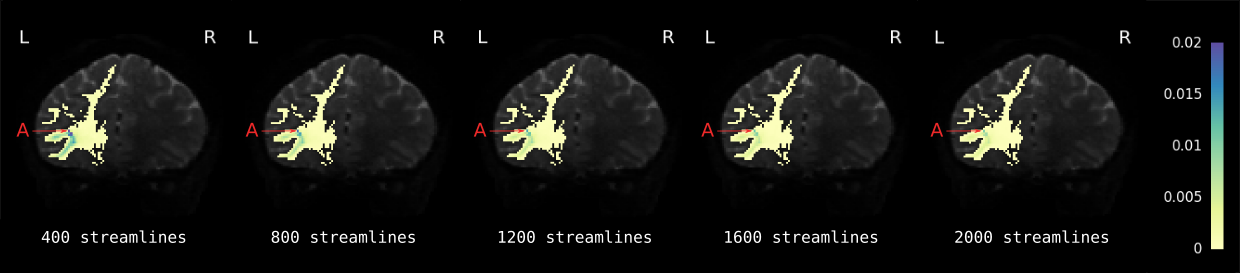
\includegraphics[width=\textwidth]{img/s1.png}
    \caption{Desviaci\'on Estandar respecto a la semilla $S1$. Mismo corte axial
             variando el tama\~no de las submuestras.}
    \label{fig:s1}
\end{figure}

\begin{figure}[h!]
   \centering
    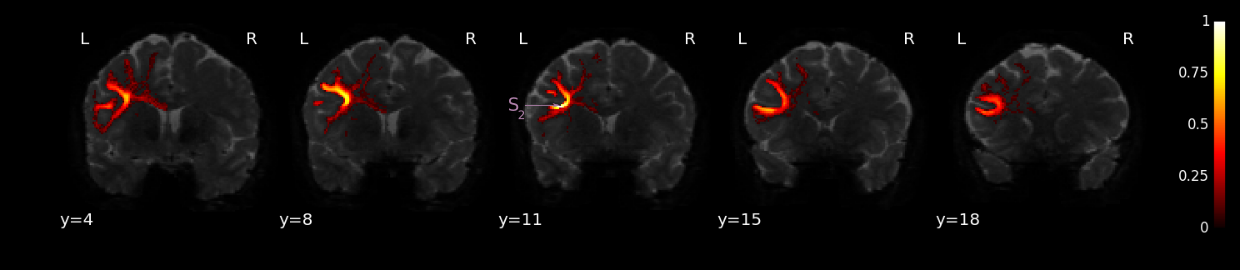
\includegraphics[width=\textwidth]{img/m2.png}
    \caption{Tractograma para la semilla $S2$ utilizando toda la muestra.}
    \label{fig:m2}
\end{figure}

\begin{figure}[h!]
   \centering
    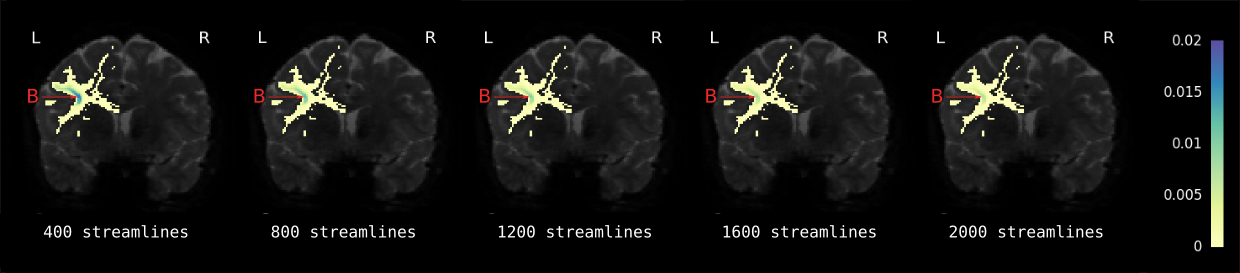
\includegraphics[width=\textwidth]{img/s2.png}
    \caption{Desviaci\'on Estandar respecto a la semilla $S2$. Mismo corte axial
             variando el tama\~no de las submuestras.}
    \label{fig:s2}
\end{figure}

\begin{figure}[h!]
   \centering
    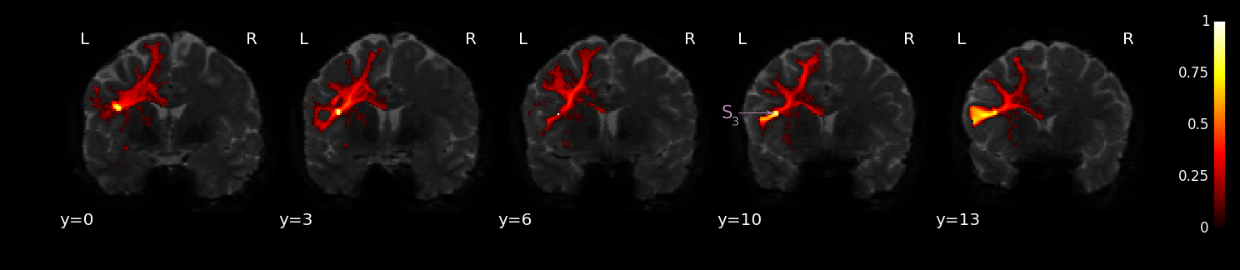
\includegraphics[width=\textwidth]{img/m3.png}
    \caption{Tractograma para la semilla $S3$ utilizando toda la muestra}
    \label{fig:m3}
\end{figure}

\begin{figure}[h!]
   \centering
    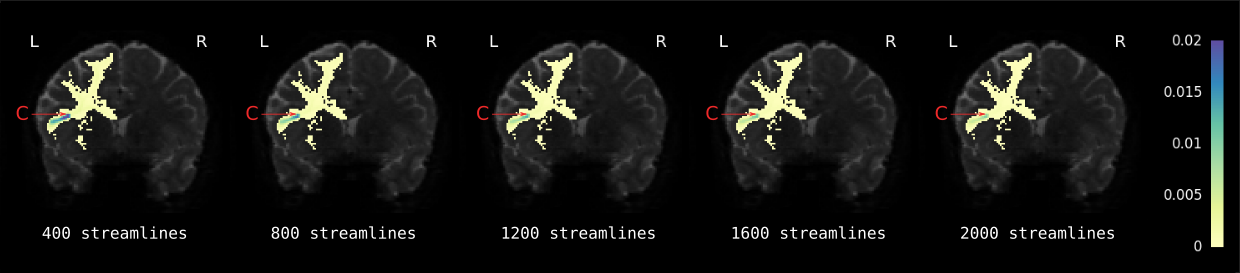
\includegraphics[width=\textwidth]{img/s3.png}
    \caption{Desviaci\'on Estandar respecto a la semilla $S3$. Mismo corte axial
             variando el tama\~no de las submuestras.}
    \label{fig:s3}
\end{figure}

\begin{figure}[h!]
   \centering
    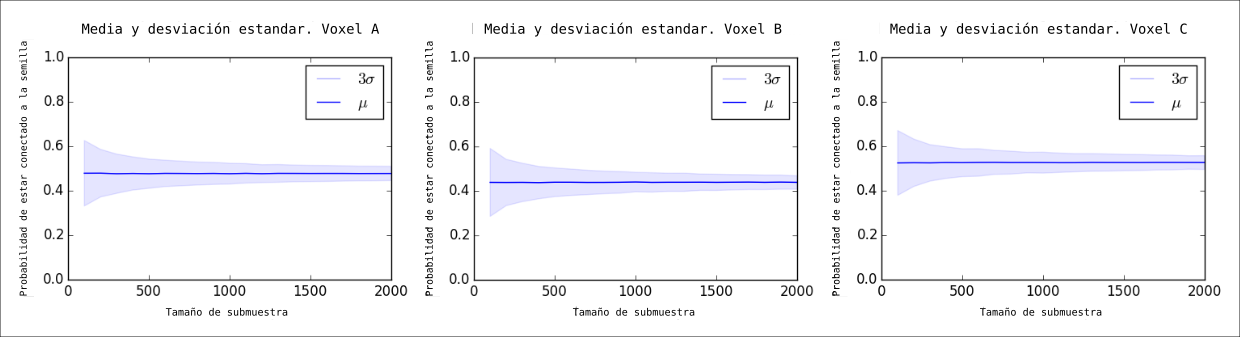
\includegraphics[width=\textwidth]{img/med_var_all.png}
    \caption{Media y desviaci\'on estandar de los voxels con mayor varianza.}
    \label{fig:mv}
\end{figure}
